\documentclass[]{article}
\setlength{\marginparwidth}{0.5in}
\usepackage{amsmath,amssymb,amsthm,mathtools,booktabs,array,tikz,pifont,comment,graphicx}
\usepackage[author-year]{amsrefs}
\input FJHDef.tex


\DeclareMathOperator{\Var}{Var}
\newcommand{\tVar}{\widetilde{\Var}}
\DeclareMathOperator{\err}{err}
\DeclareMathOperator{\maxcost}{maxcost}
\DeclareMathOperator{\mincost}{mincost}
\newcommand{\oerr}{\overline{\err}}
\newcommand{\herr}{\widehat{\err}}
\newcommand{\terr}{\widetilde{\err}}

\newtheorem{theorem}{Theorem}
\newtheorem{prop}[theorem]{Proposition}
\newtheorem{lem}{Lemma}
\newtheorem{cor}{Corollary}
\theoremstyle{definition}
\newtheorem{algo}{Algorithm}
\newtheorem{condit}{Condition}
%\newtheorem{assump}{Assumption}
\theoremstyle{remark}
\newtheorem{rem}{Remark}
\newcommand{\Fnorm}[1]{\abs{#1}_{\cf}}
\newcommand{\Gnorm}[1]{\abs{#1}_{\cg}}
\newcommand{\flin}{f_{\text{\rm{lin}}}}


\begin{document}

\title{Reliable Adaptive Quadrature for Cones of Integrands}
\author{Fred J. Hickernell, Martha Razo, and Sunny Yun}
\maketitle 


\begin{abstract} Hi
\end{abstract}


\section{Introduction} 

Although some mathematical problems can be solved using pencil and paper, many others can only be solved via numerical algorithms.  These algorithms typically generate a sequence of approximations that converge to the true solution.  The user wants to know when to stop the approximation process because the error is no greater than the specified error tolerance $\varepsilon$.  Stopping criteria for existing algorithms are based either on inconvenient assumptions or on heuristics.  

We focus on the problem of integrating cones of integrands and are able to construct a reliable error estimate for the trapezoidal rule that depends on function values.  This leads to an adaptive trapezoidal algorithm that is guaranteed to provide the value of the integral to within the desired absolute error tolerance.  In view of our new algorithm and the known flaws in of existing adaptive quadrature rules, we advocate changing how error estimation for quadrature is taught in elementary numerical analysis courses.  We also explain how our new paradigm for quadrature can be extended to other adaptive numerical algorithms.

\subsection{Why Numerical Integration Is Needed?}
There are various analytic methods for evaluating integrals, e.g., substitution, integration by parts, and partial fractions.  Unfortunately, many elementary functions have integrals that \emph{cannot} be expressed as elementary functions.  One example is the standard normal probability density, $\phi: x \mapsto \me^{-x^2/2}/\sqrt{2 \pi}$, whose integral is the standard normal distribution, $\Phi : x \mapsto \int_{-\infty}^x \phi(t) \, \dif t$.  Since the $\Phi$ is not an elementary function, values of $\Phi$ must be provided via tables in statistics textbooks and special functions in calculators. By contrast, the derivatives of elementary functions are always elementary functions.  

\subsection{The Basic Trapezoidal Rule}
To compute integrals that are not amenable to analytic methods one must turn to numerical integration (quadrature) methods such as the trapezoidal rule, $T_n$, which is often introduced in calculus courses:
\begin{equation}
\int_0^1 f(x) \, \dif x \approx T_n(f) := \frac{1}{2n} \left [ f(0) + 2 f(1/n) + \cdots + 2 f(1-1/n) + f(1) \right].
\end{equation}
The trapezoidal rule is the integral of the piecewise linear spline approximation to the integrand.  The name of the rule comes from the fact that the integral of the linear spline is a sum of areas of trapezoids (see Figure \ref{Gausstrapfig}). Under mild smoothness conditions on $f$ one observes that $T_n(f)$ approaches $\int_0^1 f(x) \, \dif x$ as $n$ increases. 

For the user's convenience one would like to turn $T_n$ into an \emph{automatic} quadrature algorithm --- one that automatically chooses $n$ to ensure that the trapezoidal rule error is small enough.  Given the user's tolerance for error, $\varepsilon$, an automatic trapezoidal algorithm should choose $n$ such that 
\begin{equation} \label{errdef}
\err(f,n) := \abs{\int_0^1 f(x) \, \dif x - T_n(f)} \le \varepsilon.
\end{equation}

Although $\err(f,n)$ is rarely known exactly, there exist rigorous upper bounds on the error that are proportional to $1/n^2$ and the roughness of the integrand, e.g., see \ocite{BraPet11a}*{Sect.\ 7.2, (7.15)}: 
\begin{equation} \label{traperrbd}
\err(f,n) \le \oerr(f,n):=\frac{\Var(f')}{8n^2}, \qquad n \in \naturals := \{1, 2, \ldots \}. 
\end{equation}
Here $\Var(\cdot)$ represents the (total) variation of a function, which is defined as
\begin{multline} \label{vardef}
\Var(f) \\
:= \sup \left \{ \sum_{i=1}^n \abs{f(x_i)-f(x_{i-1})} : n \in \naturals, \ 0 \le x_0 < x_1 < \cdots < x_{n} \le 1 \right\}.
\end{multline}
Intuitively, $\Var(f)$ is the total vertical distance up and down that one travels on a roller coaster whose track is the graph of $f$. The function $f \mapsto \Var(f')$ is a semi-norm. The trapezoidal rule gives the exact answer for linear integrands.  Error bound \eqref{traperrbd} reflects this fact since if $f(x)=ax+b$, then $f'(x)=a$, and so $\Var(f')=0$.

To illustrate this error bound, consider the normal probability example mentioned above.  The trapezoidal rule approximation using $n=4$ trapezoids, the actual error, and the error bound are as follows:
\begin{subequations} \label{GaussExample}
\begin{gather}
f(x) = 2\phi(2x) = \sqrt{\frac{2}{\pi}} \me^{-2x^2}, \qquad \int_0^1 f(x)  \, \dif x = 0.4772, \qquad T_{4}(f)= 0.4750, \\
\Var(f') = 1.5038, \qquad \err(f,4)=0.0022 \le 0.0117 = \oerr(f,4).
\end{gather}
\end{subequations}
(The value of the integral to four significant digits may be found by a variety of quadrature algorithms.)  Figure \ref{Gausstrapfig} depicts the integrand and the trapezoidal rule approximation. As expected, the actual error is bounded above by the error bound in \eqref{traperrbd}.

\begin{figure}
\centering 
\includegraphics[width=8cm]{GaussInteg4TrapFigcolor.eps}
\caption{The integrand in \eqref{GaussExample} and the trapezoidal rule approximation for the integral. \label{Gausstrapfig}}
\end{figure}

Error bound \eqref{traperrbd} can help us determine how large $n$ must be to meet the error tolerance if an upper bound on $\Var(f')$ is available. Section \ref{autoballsec} provides the details of an automatic algorithm for such cases.  Unfortunately, in practice nothing may be known a priori about $\Var(f')$. Adaptive algorithms do not require an upper bound on $\Var(f')$ but estimate the error based on the function values sampled and then apply a stopping criterion to determine how many function values are required.  Section \ref{flawstopsec} describes the stopping criterion commonly taught in numerical analysis courses, but which has significant flaws, as pointed out by James Lyness \ycite{Lyn83}.  An improved stopping criterion for integrands lying in cones is described in Section \ref{newalgosec}.  Much of this section is taken from \ocite{HicEtal14b}, which presents a general framework for guaranteed automatic algorithms and also describes the new adaptive trapezoidal algorithm presented here.  In this article we discuss in greater detail the new adaptive trapezoidal algorithm.  In Section \ref{discusssec} we discuss the ramifications of these developments for for how we teach numerical integration in calculus courses and later on.  We also discuss the how we should go about developing new numerical algorithms.


\section{An Automatic Algorithm for Balls of Integrands} \label{autoballsec}

If $f$ has a simple form, like the example in \eqref{GaussExample}, then one may be able to derive an upper bound on $\Var(f')$.  In this case the following automatic algorithm based on error bound \eqref{traperrbd} may be used.  

\begin{algo}[Automatic, for Balls] \label{ballalgo} Given a $\sigma>0$ and an error tolerance, $\varepsilon$, set 
\begin{equation}\label{algo1n}
n = \left \lceil \sqrt{\sigma/(8\varepsilon)} \right \rceil,
\end{equation}
and return the trapezoidal rule approximation $T_n(f)$ as the answer.
\end{algo}
\begin{theorem} \label{ballalgothm} If $\Var(f') \le \sigma$, then Algorithm \ref{ballalgo} is successful, i.e., 
\[
\abs{\int_0^1 f(x) \, \dif x - T_n(f)}\le \varepsilon.
\]
\end{theorem}

Algorithm \ref{ballalgo} is guaranteed to work for all integrands lying in the ball $\cb_{\sigma}=\{f : \Var(f') \le \sigma\}$.  This algorithm is automatic because it expends as much effort as required by the error tolerance, $\varepsilon$ and the radius of the ball, $\sigma$, to obtain the desired answer.  It is not an adaptive algorithm because the computational cost does not depend on the particulars of $f$.

For $f$ in \eqref{GaussExample}, one may choose $\sigma=\Var(f')=1.5038$, and then Algorithm \ref{ballalgo} uses $n = \lceil 0.4336/\sqrt{\varepsilon}\, \rceil$ trapezoids.  However, not all integrands have first derivatives whose variations are so easy to bound.  

\section{An Adaptive Trapezoidal Algorithm with a Flawed Stopping Criterion} \label{flawstopsec}

Adaptive quadrature algorithms do not require the user to specify $\sigma$.  Instead, they bound or estimate the error using only function values and then determine the sample size accordingly.  MATLAB \ycite{MAT8.1}, Mathematica \ycite{Mat9a}, NAG \ycite{NAG23}, and R \ycite{R2512} all contain automatic quadrature algorithms.  Unfortunately, their stopping criteria are unreliable, as pointed out by James Lyness \ycite{Lyn83}.  To illustrate the flawed logic that leads to unreliable error estimation in these sophisticated algorithms, we focus on the simpler case of an adaptive trapezoidal algorithm.

\subsection{A Popular Error Estimate}
Texts such as \ocite{BurFai10}*{p.\ 223--224}, \ocite{CheKin12a}*{p.\ 233}, and  \ocite{Sau12a}*{p.\ 270}, advise readers to estimate the error of $T_n(f)$ by comparing it to $T_{n/2}(f)$, specifically,
\begin{equation}\label{baderr}
\herr(f,n) = \frac{\abs{T_n(f) - T_{n/2}(f)}}{3}, \qquad \frac n2 \in \naturals.
\end{equation}
This error estimate leads to the following adaptive, automatic  quadrature algorithm. For each iteration the number of trapezoids is doubled so that the data from the previous iteration can be reused. 

\begin{algo} \label{baderralgo} Given an error tolerance, $\varepsilon$, let $j=1$ and $n_1=2$.

\begin{description} 

\item[Step 1] Compute the error estimate $\herr(f,n_j)$ according to \eqref{baderr}.

\item [Step 2] If $\herr(f,n_j) \le \varepsilon$, then return the trapezoidal rule approximation $T_{n_j}(f)$ as the answer.  

\item [Step 3] Otherwise let $n_{j+1}=2 n_j$, increase $j$ by one, and go to Step 1.

\end{description}

\end{algo}

Error estimate \eqref{baderr} may be justified by noting that Simpson's rule may be written as 
\begin{align*}
S_n(f) &:= \frac{4T_n(f) - T_{n/2}(f)}{3} =  T_n(f) + \frac{T_n(f) - T_{n/2}(f)}{3}= \\
& = \frac{1}{3n} \left [ f(0) + 4 f(1/n) + 2 f(2/n) + 4 f(3/n) + \cdots + 4 f(1-1/n) + f(1) \right].
\end{align*}
The error bound for Simpson's rule then serves as an bound on the error of $\herr(f,n)$ \cite{BraPet11a}*{Sect.\ 7.3, p.\ 231}:
\begin{align} \label{Simperrbd}
\abs{\err(f,n) - \herr(f,n)} & \le \abs{\int_0^1 f(x) \, \dif x - T_n(f) - \frac{T_n(f) - T_{n/2}(f)}{3}} \\
\nonumber
& = \abs{\int_0^1 f(x) \, \dif x - S_n(f)}  \le \frac{\Var(f''')}{36n^4}, \qquad \frac{n}2 \in \naturals. 
\end{align}
Comparing the orders of convergence in \eqref{traperrbd} and \eqref{Simperrbd}, it follows that $\herr(f,n)$ does an excellent job in approximating $\err(f,n)$ \emph{for $n$ large enough}, assuming finite $\Var(f''')$.

Unfortunately, without knowing an upper bound on $\Var(f''')$, one cannot know how large $n$ must be for $\herr(f,n)$ to be reliable.  If one really does have an upper bound on $\Var(f''')$, then it makes more sense to apply Simpson's rule and obtain a higher order convergence rate than that of Algorithm \ref{baderralgo}.  Since there is no really rigorous and compelling argument to use Algorithm \ref{baderralgo}, we do not formulate any theorem guaranteeing it.

One may identify integrands, $f$, that fool the error estimate completely, e.g.,
\begin{equation} \label{failcond}
\int_0^1 f(x) \, \dif x =  1, \quad T_{n}(f)=T_{n/2}(f) = -1, \quad \err(f,n)=2 \ne 0 = \herr(f,n).
\end{equation}
Equation \eqref{Simperrbd} implies that $\Var(f''') \ge 36 n^4 \abs{\err(f,n) - \herr(f,n)}$.  So, unless $n$ is small, any integrand $f$ satisfying \eqref{failcond} must have large  $\Var(f''')$.  Figure \ref{spikeflukefig} shows two such integrands for $n=16$. These two integrands illustrate two different ways in which the error estimate $\herr(\cdot)$ fails, and hence, Algorithm \ref{baderralgo} also fails.  One way is ultimately unavoidable but should be quantifiable.  The other way is inexcusable, but is prevalent in widely used automatic numerical quadrature.

\begin{figure}
\centering 
\includegraphics[width=5.5cm]{SpikyInteg16TrapFigcolor.eps} \qquad
\includegraphics[width=5.5cm]{FlukyInteg16TrapFigcolor.eps}
\caption{Examples of a spiky integrand (left) and a fluky integrand (right), which satisfy the failure conditions \eqref{failcond} for $n=16$. \label{spikeflukefig}}
\end{figure}

The failure of Algorithm \ref{baderralgo} cannot be solved by using a more conservative stopping criterion of the form $C\herr(f,n_j) \le \varepsilon$ in Step 2 where $C>1$.  Integrands satisfying \eqref{failcond} have an estimated error of $C\herr(f,n)=0$ regardless of how large $C$ is.

\subsection{Spiky Integrands} 

Figure \ref{spikeflukefig} (left) depicts the following spiky integrand, which satisfies \eqref{failcond}:
\begin{equation} \label{spiky}
f_{\text{spiky}}(x;n) = -1 + 60[\bbl nx \bbr(1-\bbl nx \bbr)]^2, \qquad \frac n2 \in \naturals, \quad \bbl x \bbr := x \bmod 1.
\end{equation}
The spiky integrand is constructed to be constant at the data points with spikes in between.  It has  $n+1$ local minima of $-1$, and $n$ local maxima of $11/4$.
The variation of the first and third derivatives of $f_{\text{spiky}}(\cdot;n)$ increase with $n$ as follows:
\begin{equation*}
\Var(f'_{\text{spiky}}(\cdot;n))= \frac{80n^2}{\sqrt{3}}, \qquad \Var(f'''_{\text{spiky}}(\cdot;n))= 1440n^4.
\end{equation*}

The problem of spiky integrands is not unique to Algorithm \ref{baderralgo}.  \emph{Any} quadrature algorithm that depends only on function values to estimate error will be fooled by sufficiently spiky integrands.  Suppose that the quadrature algorithm samples the integrand at a seqeunce of points, $\xi_1, \xi_2, \ldots$, and suppose that $f(\xi_i)=-1$ for all $\xi_i$.  Here the algorithm may even be adaptive, meaning that $\xi_{i+1}$ may depend on $(\xi_1, f(\xi_1)), \ldots, (\xi_i, f(\xi_i))$.  Eventually the algorithm stops.  If the algorithm is to be accurate for the constant integrand, $x \mapsto -1$, then the estimate of the integral to be $-1$ (or very close).  However, one can construct a non-constant function that shares the same data --- $f(\xi_i)=-1$ for all $\xi_i$ --- while having any value of the integral one wants. Such functions completely fool the algorithm.

Although Algorithm \ref{ballalgo} for balls of integrands can be fooled by spiky integrands, Theorem \ref{ballalgothm} remains valid because those spiky integrands lie outside the ball $\cb_{\sigma}$.  By increasing $\sigma$ one may accommodate spikier integrands.  Algorithm \ref{conealgo} in Section \ref{newalgosec} below can also be fooled by spiky integrands, however, its guarantee in Theorem \ref{conealgothm} remains valid because those spiky integrands lie outside the cone, $\cc_{\tau}$.  By increasing $\tau$ one may accommodate spikier integrands.  Moreover, the cone parameter itself corresponds to an inverse length scale corresponding to the amount of spikiness that one wishes to tolerate.

\subsection{Fluky Integrands} \label{flukysubsec}

Thirty years ago James Lyness wrote a SIAM Review article, \emph{When Not to Use an Automatic Quadrature Routine}.  While recognizing the problem of spiky integrands, he claims that there is even a more serious problem with automatic quadrature methods   \cite{Lyn83}*{p.\ 69}:
\begin{quote}
While prepared to take the risk of being misled by chance alignment of zeros in the integrand function, or by narrow peaks which are ``missed,'' the user may wish to be reassured that for ``reasonable'' integrand functions which do not have these characteristics all will be well. It is the purpose of the rest of this section to demonstrate by example that he cannot be reassured on this point. In fact the routine is likely to be unreliable in a significant proportion of the problems it faces (say $1$ to $5\%$) and there is no way of predicting in a straightforward way in which of any set of apparently reasonable problems this will happen.
\end{quote}
Lyness went on to describe how to construct a ``reasonable'' integrand that fools an automatic quadrature algorithm.  We would call this a \emph{fluky} integrand.  

Figure \ref{spikeflukefig} (right) plots a fluky integrand for Algorithm \ref{baderralgo}:
\begin{equation} \label{fluky}
f_{\text{fluky}}(x;n) = \frac{2 - 5 n^2 + n^4}{2}+ 15n^2 x(1-x)\{1 - n^2 x(1-x)\}, \qquad n \in \naturals.
\end{equation}
The integrand $f_{\text{fluky}}(\cdot;n)$ satisfies \eqref{failcond} for even $n$.   In contrast to the spiky integrand, this fluky integrand has only one local minimum of size $\Order(n^4)$ located at $1/2$ and two local maxima of size at $\Order(n^4)$ located at $\Order(n^{-2})$ and $1-\Order(n^{-2})$.  The variation of the first and third derivatives of $f_{\text{fluky}}(\cdot;n)$ increase with $n$, specifically,
\begin{equation*}
\Var(f'_{\text{fluky}}(\cdot;n))= \frac{10 n}{3}  \Bigl[9 n + 2 \sqrt{3(-2 + n^2)^3} \Bigr ], \qquad
\Var(f'''_{\text{fluky}}(\cdot;n))= 360n^4.
\end{equation*}
Disregarding its large magnitude, $f_{\text{fluky}}$ appears to quite ``reasonable''.  We describe integrands like this one as fluky because their construction is rather delicate, and they satisfy conditions \eqref{failcond} with a small number of local optima.  In this case $f_{\text{fluky}}$ was chosen to be a fourth degree polynomial --- to ensure a small number of local optima --- with symmetry about $1/2$.  The remaining coefficients were then determined uniquely by the constraints in \eqref{failcond}.  

Nearly all existing adaptive quadrature algorithms can be fooled by both spiky and fluky integrands.  Figure \ref{fig:foolquad} displays two integrands that fool MATLAB's {\tt quad} routine by satisfying \eqref{failcond}.

\begin{figure}
\centering 
\begin{tabular}{cc}
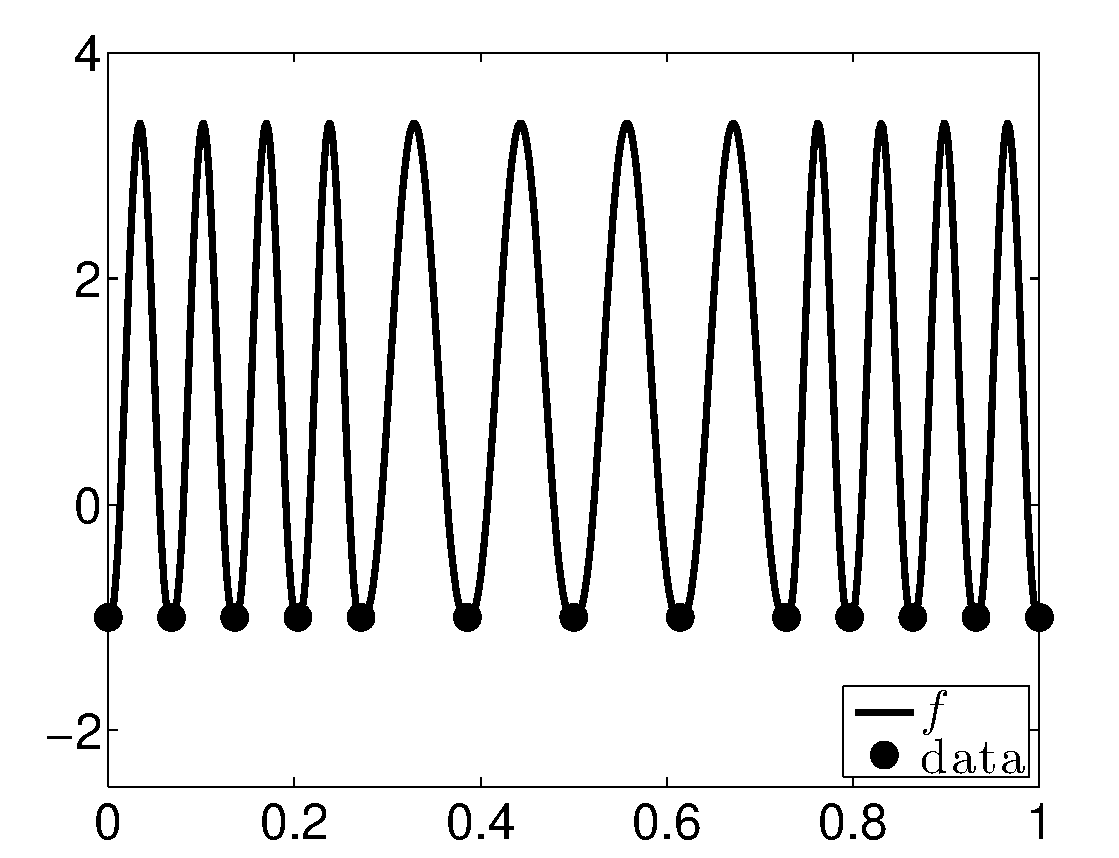
\includegraphics[width=5.5cm]{ExpositoryPaperSpikyquad.eps}
&
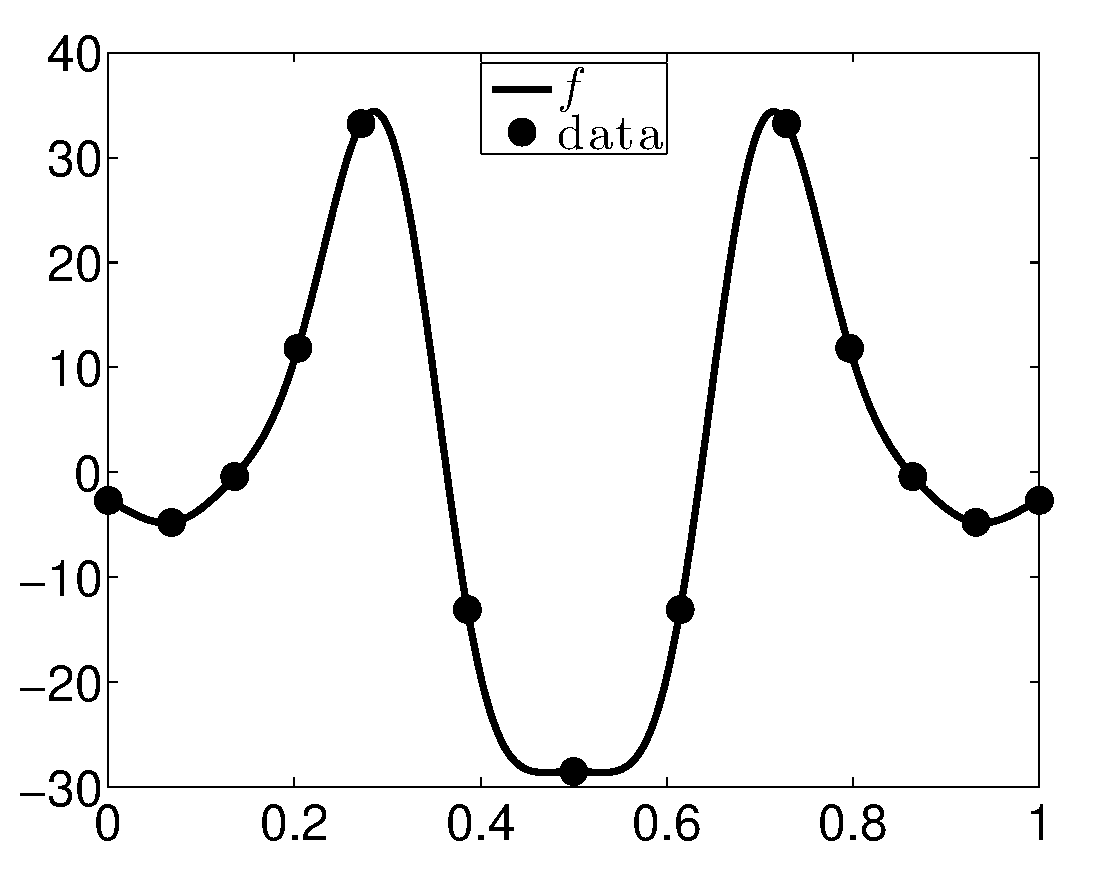
\includegraphics[width=5.5cm]{ExpositoryPaperFlukyquad.eps} \\
a) & b)
\end{tabular}
\caption{a) A spiky integrand designed to fool MATLAB's {\tt quad} and the data sampled by {\tt quad}; b) A fluky integrand designed to fool {\tt quad}. \label{fig:foolquad}}
\end{figure}

The failure of the error estimate in \eqref{baderr} for $f_{\text{fluky}}$ seems avoidable. Although the values of the trapezoidal rule are moderate, the sampled function values, $\bigl(f_{\text{fluky}}(i/n;n)\bigr)_{i=1}^{n}$ vary widely, which implies that $\Var(f_{\text{fluky}})$ must be large.  In the next section we transform this intuition into a better method for bounding the error of the trapezoidal rule.


\section{A Guaranteed, Adaptive, Automatic Trapezoidal Algorithm} \label{newalgosec}

Algorithm \ref{ballalgo} does not use any values of $f$ to determine how many trapezoids are needed to approximate the integral of $f$ because an upper bound on $\Var(f')$ is assumed.  Algorithm \ref{baderralgo} uses values of $f$ determine how how many trapezoids are needed, but in a way that allows it to detect an occurrence of large $\Var(f')$.  In this section we present a way for reliably estimating $f'$, which then can be used to construct a reliable stopping criterion for an adaptive trapezoidal algorithm.

Estimating $\Var(f')$ reliably and directly requires additional smoothness assumptions on $f$, but if we assume more smoothness, then we ought to use a different rule, like Simpson's rule.  On the other hand, knowing that $\Var(f')$ is finite does allow us to reliably estimate, a weaker semi-norm of $f$, such as $\Var(f)$.  As observed in Section \ref{flukysubsec} above, the fluky algorithms that fool Algorithm \ref{baderralgo} not only have large $\Var(f')$ but also large $\Var(f)$.  The approach taken in this section is to explore what can be accomplished by estimating a weaker semi-norm.

Let $A_n$ denote the linear spline approximation using $n+1$ equally spaced points, i.e., 
\begin{equation}
\label{Andef}
A_n(f)(x) = \begin{cases} f(0)(1-nx) + f(1/n)nx, & 0 \le x < 1/n, \\
f(1/n)(2-nx) + f(2/n)(nx-1), & 1/n \le x < 2/n, \\
\qquad \qquad \qquad \qquad \vdots & \qquad \quad \vdots \\
f(1-1/n)(n-nx) + f(1)(nx-n + 1), & 1-1/n \le x \le 1.
\end{cases}
\end{equation}   
The trapezoidal rule can be written as $T_n(f) = \int_0^1 A_n(f)(x) \, \dif x$.  Using this definition of linear spline we focus on the semi-norm defined by $f \mapsto \Var(f-A_1(f))$.  Like $f \mapsto \Var(f')$ this weaker semi-norm also vanishes for functions that are linear in $x$.  If $\Var(f')$ is finite, then it follows that $\Var(f) = \norm[1]{f'}:=\int_0^1 \abs{f(x)} \, \dif x$, so the weaker semi-norm may be written as $f \mapsto \norm[1]{f'-f(1)+f(0)}$.  It is shown in \ocite{HicEtal14b}*{Section 5.1} that 
\begin{equation} \label{weaknorm}
2 \norm[1]{f'-f(1)+f(0)} \le \Var(f') \qquad \forall f \text{ with } \Var(f')<\infty.
\end{equation}

The data-driven quantity 
\begin{equation} \label{weaknormalgo}
\norm[1]{A_n(f)'-f(1)+f(0)}= \sum_{i=1}^n \abs{f\left(\frac in \right)-f\left(\frac{i-1}n \right) - \frac{f(1)-f(0)}{n}}
\end{equation}
always underestimates $\norm[1]{f'-f(1)+f(0)}$, but not by much provided that $\Var(f')$ is not too large. Again in \ocite{HicEtal14b}*{Section 5.1} it is shown that 
\begin{equation} \label{errweaknorm}
0 \le \norm[1]{f'-f(1)+f(0)} - \norm[1]{A_n(f)'-f(1)+f(0)} \le \frac{\Var(f')}{2n}.
\end{equation}

At this point it seems that we have reached a dead end because we have an error bound in terms of $\Var(f')$, just like the trapezoidal rule error bound \eqref{traperrbd}.  However, we make a further assumption that $f$ lies in the cone defined as 
\begin{equation} \label{conedef}
\cc_{\tau} := \{f : \Var(f') \le \tau \norm[1]{f'-f(1)+f(0)} \}.
\end{equation}
This cone consists of functions whose stronger semi-norms are not too much greater than their weaker semi-norms.  The set $\cc_{\tau}$ is called a cone because $f \in \cc_{\tau}$ implies that $cf \in \cc_{\tau}$ for all $c \in \reals$.  Substituting this upper bound on $\Var(f')$ into \eqref{errweaknorm} and re-arranging the terms implies a data-driven upper bound on  $\Var(f')$:
\begin{multline} \label{varfprimeless}
\Var(f') \le \tau \norm[1]{f'-f(1)+f(0)}  \\
\le \frac{\tau \norm[1]{A_n(f)'-f(1)+f(0)}}{1-\tau/(2n)} \qquad \forall f \in \cc_{\tau},
\end{multline}
provided that $n>\tau/2$.  There is also a companion bound in the other direction based on \eqref{weaknorm} and \eqref{errweaknorm}:
\begin{equation} \label{varfprimegreat}
\norm[1]{A_n(f)'-f(1)+f(0)} \le \norm[1]{f'-f(1)+f(0)} \le \frac{\Var(f')}{2}.
\end{equation}

Plugging \eqref{varfprimeless} into \eqref{traperrbd} yields the following guaranteed error bound for the trapezoidal rule:
\begin{equation} \label{guarerr}
\err(f,n) \le \terr(f,n) := \frac{\tau \norm[1]{A_n(f)'-f(1)+f(0)}} {4n(2n-\tau)} \qquad \forall f \in \cc_{\tau}.
\end{equation}
This new error bound can then be used to construct the following adaptive, automatic quadrature algorithm, which is a simplification of \ocite{HicEtal14b}*{Algorithm 4}:

\begin{algo}[Adaptive, Automatic, for Cones] \label{conealgo} Given $\tau>0$, and an error tolerance, $\varepsilon$, let $j=1$ and $n_1=\lceil (\tau+1)/2 \rceil$.

\begin{description} 

\item[Step 1] Compute the error estimate $\terr(f,n_j)$ according to \eqref{guarerr}.

\item [Step 2] If $\terr(f,n_j) \le \varepsilon$, then return the trapezoidal rule approximation $T_{n_j}(f)$ as the answer.  

\item [Step 3] Otherwise let $n_{j+1}=2 n_j$, increase $j$ by one, and go to Step 1.

\end{description}
\end{algo}

Error bound \eqref{guarerr} is used to prove that Algorithm \ref{conealgo} is successful for integrands in $\cc_{\tau}$.  Let $N(f,\varepsilon,\tau)$ denote the eventual number of trapezoids required by this algorithm.  Because the algorithm is adaptive, the number of trapezoids depends on the particulars of $f$ as well as the error tolerance.  The two bounds \eqref{varfprimeless} and \eqref{varfprimegreat} may be used to derive both lower and upper bounds on $N(f,\varepsilon,\tau)$:

\begin{theorem}\cite{HicEtal14b}*{Theorem 7} \label{conealgothm}
Let $N(f,\varepsilon,\tau)$ denote the final $n_j$ in Algorithm \ref{conealgo}.  Then this algorithm is successful for all functions in $\cc_{\tau}$,  i.e.,  $\abs{\int_0^1 f(x) \, \dif x - T_{N(f,\varepsilon,\tau)}(f)} \le \varepsilon$.  Moreover, $N(f,\varepsilon,\tau)$ is bounded below and above as follows:
\begin{multline}
\max \left(\left \lceil\frac{\tau+1}{2} \right \rceil, \left \lceil \sqrt{\frac{ \Var(f')}{8\varepsilon}} \right \rceil \right) \\
\le \max \left(\left \lceil\frac{\tau+1}{2} \right \rceil, \left \lceil \sqrt{\frac{\tau \norm[1]{f'-f(1)+f(0)}}{8\varepsilon}} \right \rceil \right) \\
\le
N(f,\varepsilon,\tau) \\
\le \sqrt{\frac{\tau \norm[1]{f'-f(1)+f(0)}}{2\varepsilon}} + \tau + 3
\le \sqrt{\frac{\tau \Var(f') }{4\varepsilon}} + \tau + 3.
\end{multline}
\end{theorem}

Note that the cost of the algorithm depends on $\Var(f')$, but without the algorithm needing to know $\Var(f')$ in advance.   Comparing the two error bounds on which Algorithms \ref{ballalgo} and \ref{conealgo} are based and applying the , we note that 
\begin{equation*}
\frac{\Var(f')}{\sigma} \le
\frac{\terr(f,n)}{\oerr(f,n)}
\le \frac{\tau\Var(f')}{\sigma (2-\tau/n)}.
\end{equation*}



For an integrand like \eqref{GaussExample} where $\Var(f')$ is known, the number of trapezoids required by Algorithm \ref{conealgo} is no greater than  $\sqrt{\tau \Var(f') /(4\varepsilon)} + \tau + 3$, whereas for Algorithm \ref{ballalgo} with $\sigma=\Var(f')$ the number of trapezoids is no more than $\bigl \lceil \sqrt{\Var(f') /(8\varepsilon)} \, \bigr\rceil$.  The extra cost for Algorithm \ref{newalgo} comes in the form of the factor $\sqrt{2\tau}$ and the additional additive term of $\tau+1$.  On the other hand, if $\Var(f')$ is not known in advance, then the disadvantage of Algorithm  \ref{ballalgo} is that if $\Var(f')$ is not known in advance, and $\sigma$ is chosen conservatively, then Algorithm \ref{newalgo} could cost arbitrarily more than $\sqrt{\Var(f') /(8\varepsilon)}+1$ in the limit of , 

\section{Acknowledgements}  The authors are grateful for discussions with a number of colleagues. This research is supported in part by grant NSF-DMS-1115392.

\bibliography{FJH22,FJHown22}
\end{document}

The Bernoulli polynomials are described by \ocite{AbrSte64}*{Chap.\ 23, \url{http://dlmf.nist.gov/24}}.  The first six are defined as follows 
\begin{subequations} \label{Bernoulli}
\begin{gather} 
B_0(x) = 1, \qquad B_1(x) = x-1/2,  \qquad 
B_2(x)=1/6 - x(1-x), \\ 
B_3(x) = \frac{1}{2} x(1-x)(1-2x), \qquad B_4(x) = -1/30 + [x(1-x)]^2, \\
B_5(x) = \frac{1}{6} x(1-x)(1-2x)(1 + 3 x - 3 x^2).
\end{gather}
\end{subequations}

\subsection{Necessary Conditions for Failure of the Error Estimate} 
Integrands that satisfy \eqref{failcond} and fool the error estimate in \eqref{baderr} must satisfy certain conditions.  First note that the error bound in \eqref{traperrbd} implies that
\[
\Var(f') \ge 8n^2 \err(f,n) =  16n^2 \asymp n^2 \qquad \text{as } n \to \infty,
\]
so the total variation of the first derivative must be increasingly large as the number of trapezoids increases.  Moreover, the trapezoidal rule added to the error estimate in \eqref{baderr} is actually Simpson's rule:
\begin{align*}
S_n(f) &:= T_n(f) + \herr(f,n) = \frac{4T_n(f) - T_{n/2}(f)}{3} \\
& = \frac{1}{3n} \left [ f(0) + 4 f(1/n) + 2 f(2/n) + 4 f(3/n) + \cdots + 4 f(1-1/n) + f(1) \right].
\end{align*}
The error bound of Simpson's rule then serves as an bound on the error of the error estimate \cite{BraPet11a}*{Sect.\ 7.3, p.\ 231}:
\begin{equation} \label{Simperrbd}
\abs{\err(f,n) - \herr(f,n)} = \abs{\int_0^1 f(x) \, \dif x - S_n(f)} \le \frac{\Var(f''')}{36n^4}, \qquad \frac{n}2 \in \naturals. 
\end{equation}
So, integrands satisfying \eqref{failcond} must also satisfy
\[
\Var(f''') \ge 36n^4 \abs{\err(f,n) - \herr(f,n)} =  36n^4 \asymp n^4 \qquad \text{as } n \to \infty.
\]
Thus, the total variation of the third derivative must increase even faster than the minimum increase of $\Var(f')$ as the number of trapezoids increases.

The derivatives of Bernoulli polynomials are multiples of lower degree Bernoulli polynomials and the integrals of nonconstant Bernoulli polynomials vanish (see \ocite{AbrSte64}*{Chap.\ 23, \url{http://dlmf.nist.gov/24}}):
\[
B'_n(x) = n B_{n-1}(x), \quad \int_0^1 B_{n+1}(x) \, \dif x, \qquad n \in \naturals.
\]
The formula for the derivatives facilitates the computation of the total variation of the spiky and fluky examples above, confirming that the variations of their first and third derivatives satisfy the above inequalities.  For the spiky integrand defined in \eqref{spiky},
\begin{subequations} \label{spikyvariation}
\begin{gather}
%f'_{\text{spiky}}(x;n) = 240 n B_3(\bbl nx \bbr), \qquad f''_{\text{spiky}}(x;n) = 720 n^2 B_2(\bbl nx \bbr), \\ f'''_{\text{spiky}}(x;n) = 1440 n^3 B_1(\bbl nx \bbr), \\
\Var(f_{\text{spiky}}(\cdot;n))= \frac{15n}{2}, \qquad  \Var(f'_{\text{spiky}}(\cdot;n))= \frac{80n^2}{\sqrt{3}} > 16 n^2, \\
\Var(f''_{\text{spiky}}(\cdot;n))= 360n^3, \qquad \Var(f'''_{\text{spiky}}(\cdot;n))= 1440n^4 > 36n^4.
\end{gather}
\end{subequations} 
For the fluky integrand defined in \eqref{fluky},
\begin{subequations} \label{spikyvariation}
\begin{gather}
%f'_{\text{fluky}}(x;n) = - 30 n^2 [B_1(x) + 2 n^2 B_3(x)], \\ f''_{\text{fluky}}(x;n) = -30 n^2 [1 + 6 n^2 B_2(x)], \qquad f'''_{\text{fluky}}(x;n) = -360 n^4 B_1(x), \\
\Var(f_{\text{fluky}}(\cdot;n))= \frac{15}{8} (8 - 4 n^2 + n^4),  \\
\Var(f'_{\text{fluky}}(\cdot;n))= \frac{10 n}{3}  \Bigl[9 n + 2 \sqrt{3(-2 + n^2)^3} \Bigr ]  > 16 n^2, \\
\Var(f''_{\text{fluky}}(\cdot;n))= 90n^4, \qquad \Var(f'''_{\text{fluky}}(\cdot;n))= 360n^4 > 36n^4.
\end{gather}
\end{subequations}  

For the spiky integrand the asymptotic order of the total variation for large $n$ increases with the order of the derivative while for the fluky integrand it stays the same.  Specifically,
\[
\Var(f^{(j)}_{\text{spiky}}(\cdot;n)) \asymp n^{j+1}, \quad \Var(f^{(j)}_{\text{fluky}}(\cdot;n)) \asymp n^{4}, \qquad j=0, \ldots, 3.
\]
This difference in asymptotic behaviors distinguishes whether a better error bound developed in the next section will be successful:  no for the spiky integrand , but yes for the fluky integrand.
